
% По умолчанию используется шрифт 14 размера. Если нужен 12-й шрифт, уберите опцию [14pt]
\documentclass[14pt]{matmex-diploma-custom}
\usepackage{graphicx}
\usepackage{float}
\graphicspath{ {./images/} }

\begin{document}
\filltitle{ru}{
    chair              = {Математико-механический факультет},
    title              = {Разработка кулинарного Android-приложения: база данных, отображение результатов поиска рецептов},
    % Здесь указывается тип работы. Возможные значения:
    %   coursework - Курсовая работа
    %   diploma - Диплом специалиста
    %   master - Диплом магистра
    %   bachelor - Диплом бакалавра
    type               = {diploma},
    position           = {студента},
    group              = 244,
    author             = {Паршин Максим Алексеевич},
    supervisorPosition = {к.\,т.\,н., доцент},
    supervisor         = {Литвинов Ю.\,В.},
%    reviewerPosition   = {ст. преп.},
%    reviewer           = {Привалов А.\,И.},
%    chairHeadPosition  = {д.\,ф.-м.\,н., профессор},
%    chairHead          = {Хунта К.\,Х.},
%   university         = {Санкт-Петербургский Государственный Университет},
%   faculty            = {Математико-механический факультет},
%   city               = {Санкт-Петербург},
%   year               = {2013}
}
\maketitle
\tableofcontents

\section*{Введение}

Целью большого числа мобильных приложений ввиду их доступности и простоты часто является облегчение быта пользователя, в том числе и процесса приготовления пищи. Выбор блюда для приготовления, к примеру, становится проще при наличии доступа к базам данных с рецептами, который предоставляют многие приложения. При этом для эффективного поиска рецептов важно иметь возможность фильтрации по такому параметру как необходимые ингредиенты. На данный момент существует несколько русскоязычных Android-приложений, обладающих таким функционалом, но имеющих недостаток в виде недружественного пользователю интерфейса, затрудняющего работу с ними.

Цель проекта --- разработать приложение для операционной системы Android, имеющее функцию поиска кулинарных рецептов по входящим в них ингредиентам, а также другим параметрам, и интуитивно-понятный интерфейс.

\section*{Постановка задачи}
Для достижения цели перед автором были поставлены следующие задачи:

\begin{itemize}  
\item Выбрать СУБД для взаимодействия с базой данных рецептов
\item Разработать архитектуру базы данных
\item Реализовать инструмент для заполнения базы тестовыми данными
\item Реализовать механизм доступа к данным
\item Разработать элементы интерфейса для отображения результатов поиска
\end{itemize}

\section*{Обзор существующих решений}
При исследовании доступных в Google Play русскоязычных кулинарных приложений было найдено только две программы, обладающих функцией поиска рецепта по необходимым ингредиентам: <<Что готовим?>> \cite{chtogotovim} и <<Подбери рецепт>> \cite{podberi}.
\subsection*{Приложение <<Что готовим?>>}
Поиск рецептов по ингредиентам в данном приложении осуществляется путем заполнения пользователем раздела <<Холодильник>> элементами имеющихся у него продуктов и формирования по ним поискового запроса. В окне результатов поиска доступна фильтрация по сложности приготовления блюда и его типу, для каждого из рецептов отображается общее число необходимых и число совпавших с заданными ингредиентов, но сортировка по этому критерию не происходит. На странице отдельного рецепта содержится инструкция по приготовлению, а также информация о времени приготовления и количестве ингредиентов.
 \subsection*{Приложение <<Подбери рецепт>>}
 Интерфейс выбора необходимых ингредиентов в данном приложении доступен пользователю сразу при запуске. Имеются изображения для каждого ингредиента. В окне результатов поиска для каждого найденного рецепта отображается только число совпавших ингредиентов, но не общее их число в блюде. Доступна фильтрация по типу блюда. На странице рецепта можно найти инструкцию по приготовлению, информацию о количестве ингредиентов, времени приготовления и пищевой ценности.
При этом страница оформлена достаточно броско, что может затруднять комфортное использование.\\

 Подводя итог, можно сказать, что данные приложения, несмотря на наличие функциональности, достаточной для использования в быту, имеют недостатки в виде отсутствия информации о числе порций, на которое рассчитан рецепт, и принадлежности к национальной кухне, а также относительно сложного в освоении интерфейса в случае приложения <<Что готовим?>> и затрудняющего восприятие оформления в <<Подбери рецепт>>.
 
 \section*{Обзор использованных инструментов}
 \subsection*{Realm}
 Требуемую функциональность приложения было бы невозможно реализовать без базы данных с рецептами, поэтому важной задачей стал выбор подходящей СУБД. При этом ввиду отсутствия возможности разместить базу данных на удаленном сервере было принято решение хранить информацию о рецептах в локальной базе данных на устройстве, предварительно заполненной на другой платформе и перенесенной в приложение.
 
С учетом современных тенценций в мобильной разработке, как возможные альтернативы были рассмотрены реляционная СУБД SQLite (и ORM-технологии) и появившаяся сравнительно недавно объектно-ориентированная NoSQL база данных Realm, которая в итоге и была выбрана для использования в проекте. Основным аргументом в пользу этой СУБД стала возможность быстрой интеграции базы данных, заполненной с помощью десктопного приложения, в Android-приложение без необходимости изучения двух ORM-технологий для разных платформ, что увеличило бы время работы над проектом. Realm имеет одинаковый механизм доступа к объектам данных на всех поддерживаемых платформах, и для интеграции базы в Android-приложение в его коде потребовалось лишь определить такие же классы-сущности, как при её заполнении, и затем обращаться к данным с помощью них.

Что касается скорости работы, согласно исследованию, проведенному пользователем GitHub с именем аккаунта AlexeyZatsepin \cite{realmbenchmark}, Realm показывает сравнимое с другими технологиями время чтения из базы данных и с большим отрывом (Рис. \ref{realmwrite}) опережает их по времени записи. 

\begin{figure}[h]
\centering
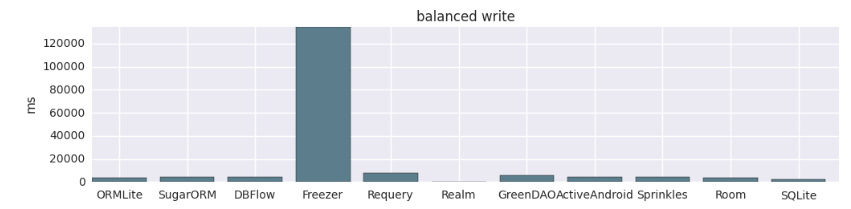
\includegraphics[width=\textwidth]{balanced_write.png}
\caption{Сравнение времени выполнения операции записи для популярных мобильных баз данных}
\label{realmwrite}
\end{figure}

\subsection*{AngleSharp}

Для апробации разрабатываемого приложения требовалось заполнить базу тестовыми данными, поэтому было принято решение реализовать отдельный инструмент, задачей которого было бы получение информации о рецептах с некоторого веб-сайта. Так как эта вспомогательная программа сама по себе не использовалась бы при эксплуатации Android-приложения, написанного на Kotlin, она была вынесена в отдельный десктопный модуль. Языком разработки стал C\#, опытом программирования на котором обладал автор. Чтобы извлечь определенные данные о рецепте из исходного кода веб-страницы, потребовалось воспользоваться одной из библиотек для парсинга HTML-разметки. После изучения исследования популярных инструментов, проведенного пользователем портала habr.com Павлом Носовичем \cite{anglesharp} и показавшего, что библиотека AngleSharp обладает рядом преимуществ, таких как возможность использования CSS-селекторов, было решено использовать именно её.

\section*{Реализация}


\subsection*{Парсер}

При разработке вспомогательного приложения-парсера HTML-разметки требовалось обеспечить возможность его расширения для работы с различными сайтами и организовать единый интерфейс доступа к информации, содержащейся на страницах с рецептами, для каждого из них. Чтобы решить данную задачу, была спроектирована и реализована следующая архитектура классов (Рис. \ref{parser}):

\begin{itemize}  
\item \textbf{Интерфейс IParsingLogic} Данный интерфейс наследуется для работы с отдельным веб-сайтом. Для каждого элемента данных о рецепте, например, времени приготовления, реализуется метод, с помощью библиотеки AngleSharp извлекающий эти данные из HTML-разметки переданной страницы.
\item \textbf{Класс ParsingContext} При обработке страниц для некоторых сайтов может быть необходимо учитывать не только информацию о рецепте, содержащуюся непосредственно на них, но и информацию, определяемую по разделу сайта, где страница находится. К примеру, на странице с рецептом может быть не указано, что он относится к итальянской кухне, но по тому факту, что страница находится в разделе "Итальянская кухня", эту информацию можно выяснить. В таком случае можно унаследовать класс ParsingContext для раздела итальянской кухни и переопределить метод GetCuisine(), чтобы он возвращал название <<итальянская>>. Остальные же методы будут просто вызывать соответствующие методы переданного им экземпляра IParsingLogic. Также класс ParsingContext содержит метод GetPages(), возвращающий коллекцию строк адресов страниц, относящихся к данному разделу.
\item \textbf{Интерфейс IParserFactory} Реализуется для отдельного сайта и позволяет объединить всю логику работы с ним в одной сущности. 
\item \textbf{Класс RecipeParser} Используя переданный в конструкторе экземпляр IParserFactory осуществляет обход по страницам разделов определенного сайта, извлекает информацию о рецептах и обращается к классу, работающему с базой данных, для сохранения полученных рецептов.

\end{itemize}

\begin{figure}[h]
\centering
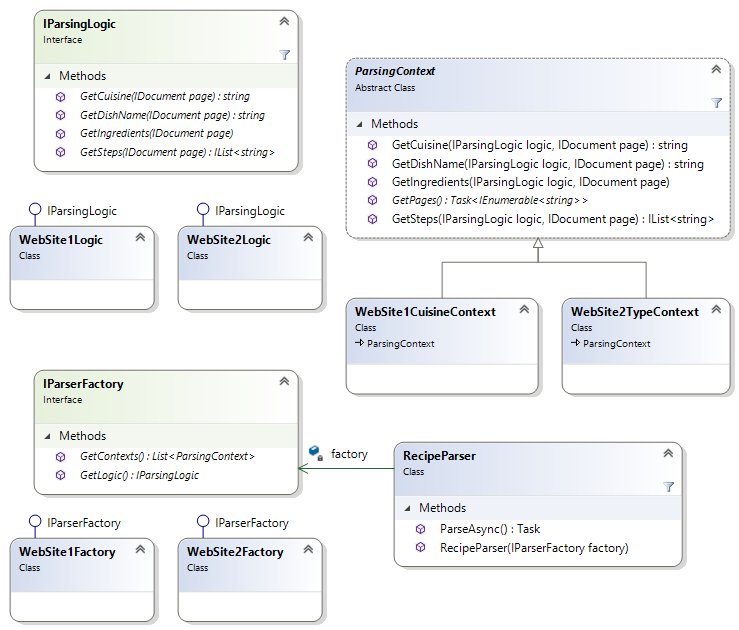
\includegraphics[width=\textwidth]{parser.png}
\caption{Диаграмма классов парсера}
\label{parser}
\end{figure}

\subsection*{База данных}

Для хранения информации о рецептах была реализована архитектура, состоящая из трех классов (Рис. \ref{database}), наследующих RealmObject --- базовый класс Realm, представляющий отдельную сущность в базе данных (аналогично таблице в реляционных СУБД):

\begin{figure}[h]
\centering
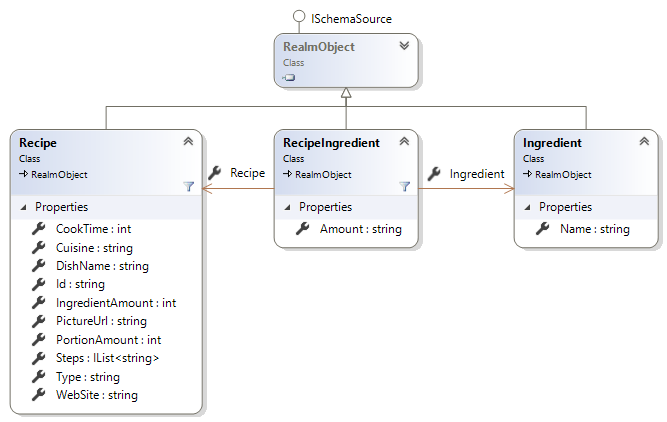
\includegraphics[width=\textwidth]{database.png}
\caption{Диаграмма классов базы данных}
\label{database}
\end{figure}

\begin{itemize}  
\item \textbf{Recipe} Объекты данного класса содержат информацию об отдельном рецепте: название блюда, шаги приготовления, число порций, принадлежность к национальной кухне и т. д.
\item \textbf{Ingredient} Класс, представляющий ингредиент, который может содержаться в блюде. Имеет свойство Name, возвращающее название ингредиента.
\item \textbf{RecipeIngredient} Класс, используемый для представления связи между рецептами и необходимыми для приготовления ингредиентами. Имеет свойства Recipe и Ingredient, возвращающие ссылки соответственно на рецепт блюда и конкретный его ингредиент. Свойство Amount предоставляет информацию о количестве, в котором ингредиент должен использоваться.
\end{itemize}

\begin{figure}[h]
\centering
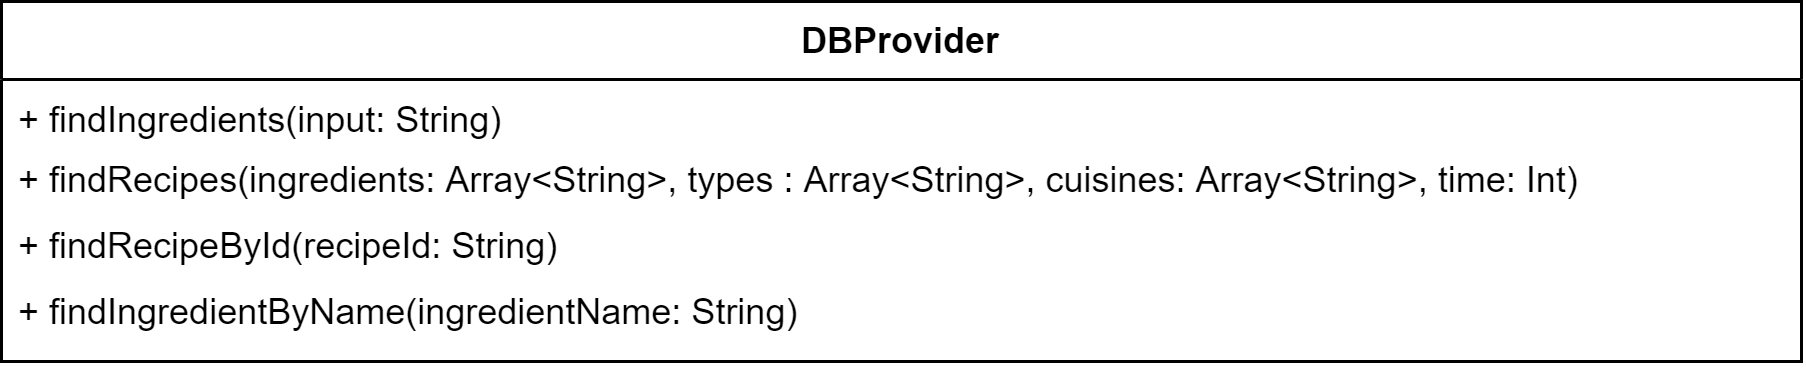
\includegraphics[width=\textwidth]{dbandroid.png}
\caption{Класс DBProvider, используемый в Android-приложении (Kotlin)}
\label{dbandroid}
\end{figure}

\begin{figure}[h]
\centering
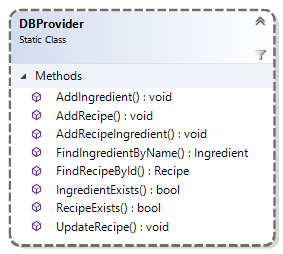
\includegraphics{dbparser.png}
\caption{Класс DBProvider, используемый в парсере (C\#)}
\label{dbparser}
\end{figure}

Описанная архитектура используется для взаимодействия с данными как в парсере, так и в Android-приложении. 

Для осуществления операций с базой данных, таких как поиск рецептов по параметрам и запись новых рецептов в базу, в обоих модулях реализованы служебные классы DBProvider (Рис. \ref{dbparser} и \ref{dbandroid}). 


\subsection*{Отображение результатов поиска}

Отображение найденных рецептов в мобильном приложении на Kotlin осуществляется с помощью фрагментов --- стандартных компонентов Android API, представляющих собой модули, имеющие пользовательский интерфейс и содержащие логику взаимодействия с ним \cite{fragments}. Реализация пользовательских фрагментов производилась путем наследования от класса Fragment и переопределения методов, связанных с <<жизненным циклом>> фрагмента, таких как OnCreate(), который вызывается при создании фрагмента приложением. С каждым фрагментом связан .xml файл, описывающий его графическое представление.

\begin{figure}[h]
\centering
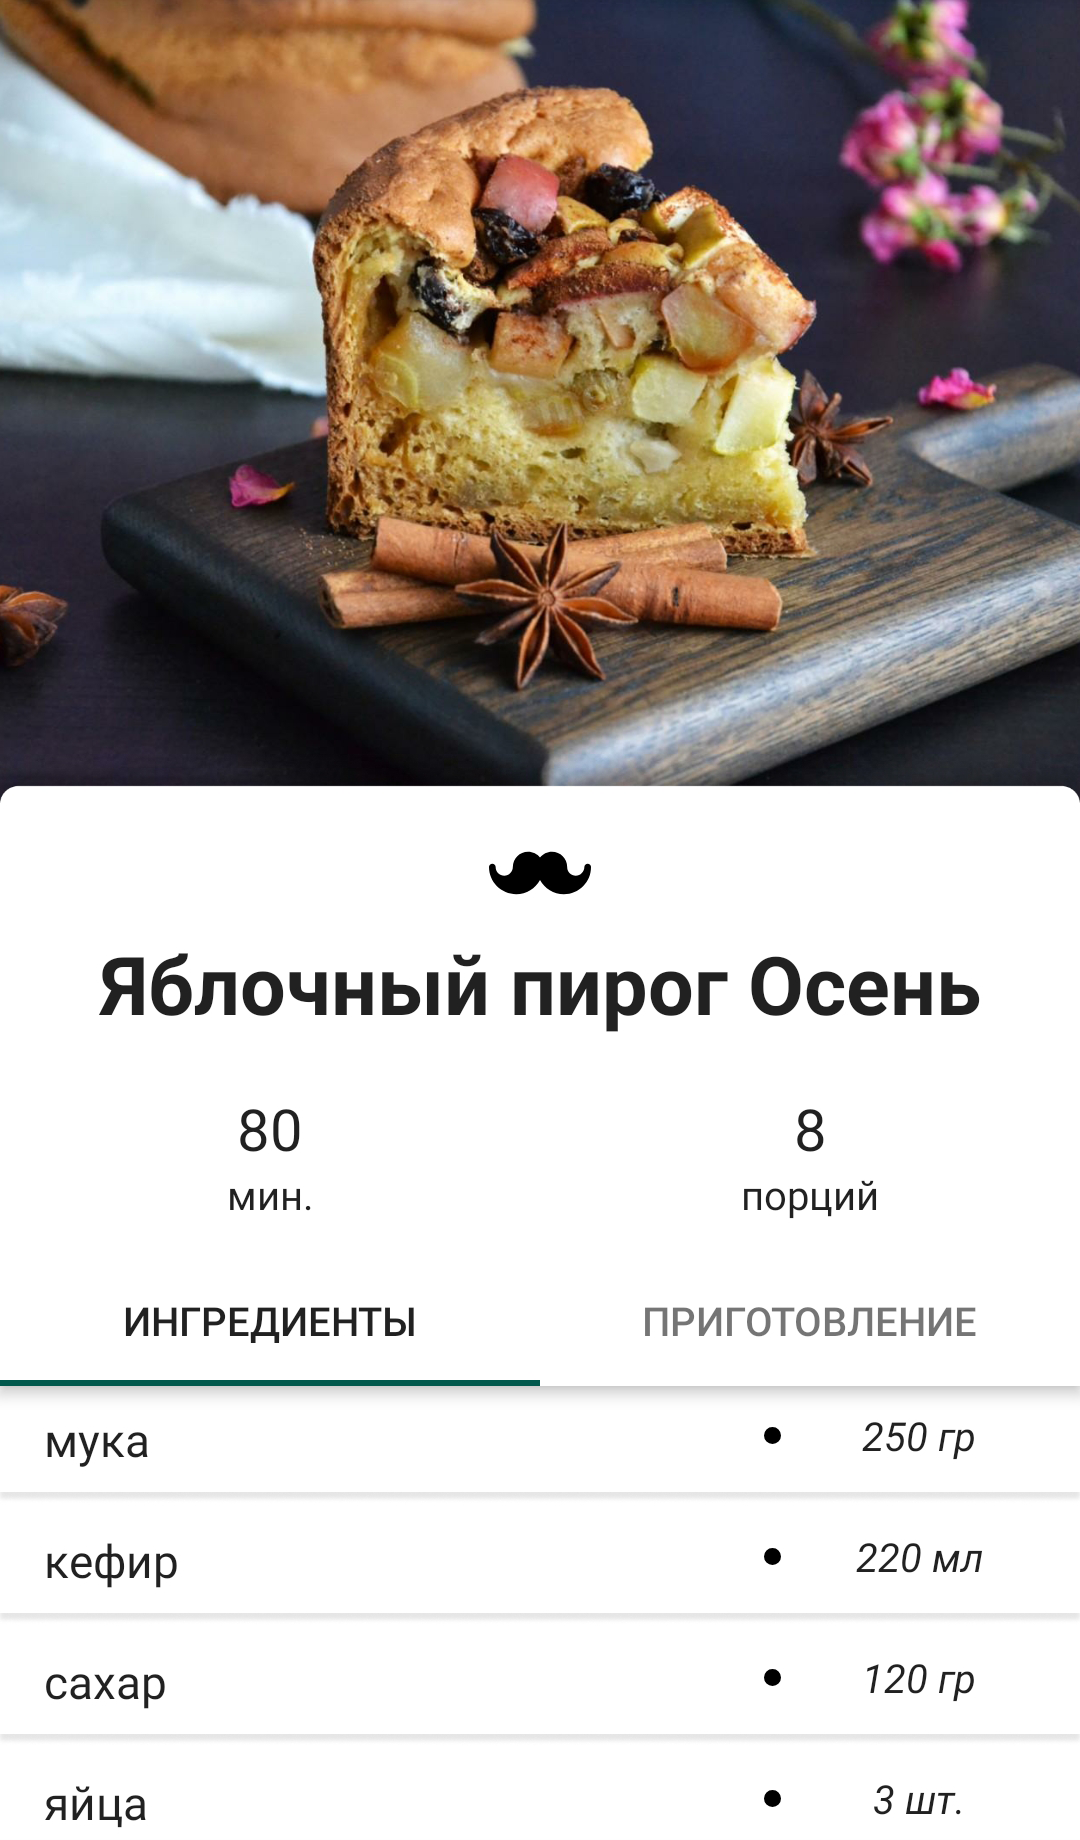
\includegraphics[scale=0.15]{recipepage.png}
\caption{Графический интерфейс фрагмента RecipeFragment}
\label{recipepage}
\end{figure}

\begin{figure}[h]
\centering
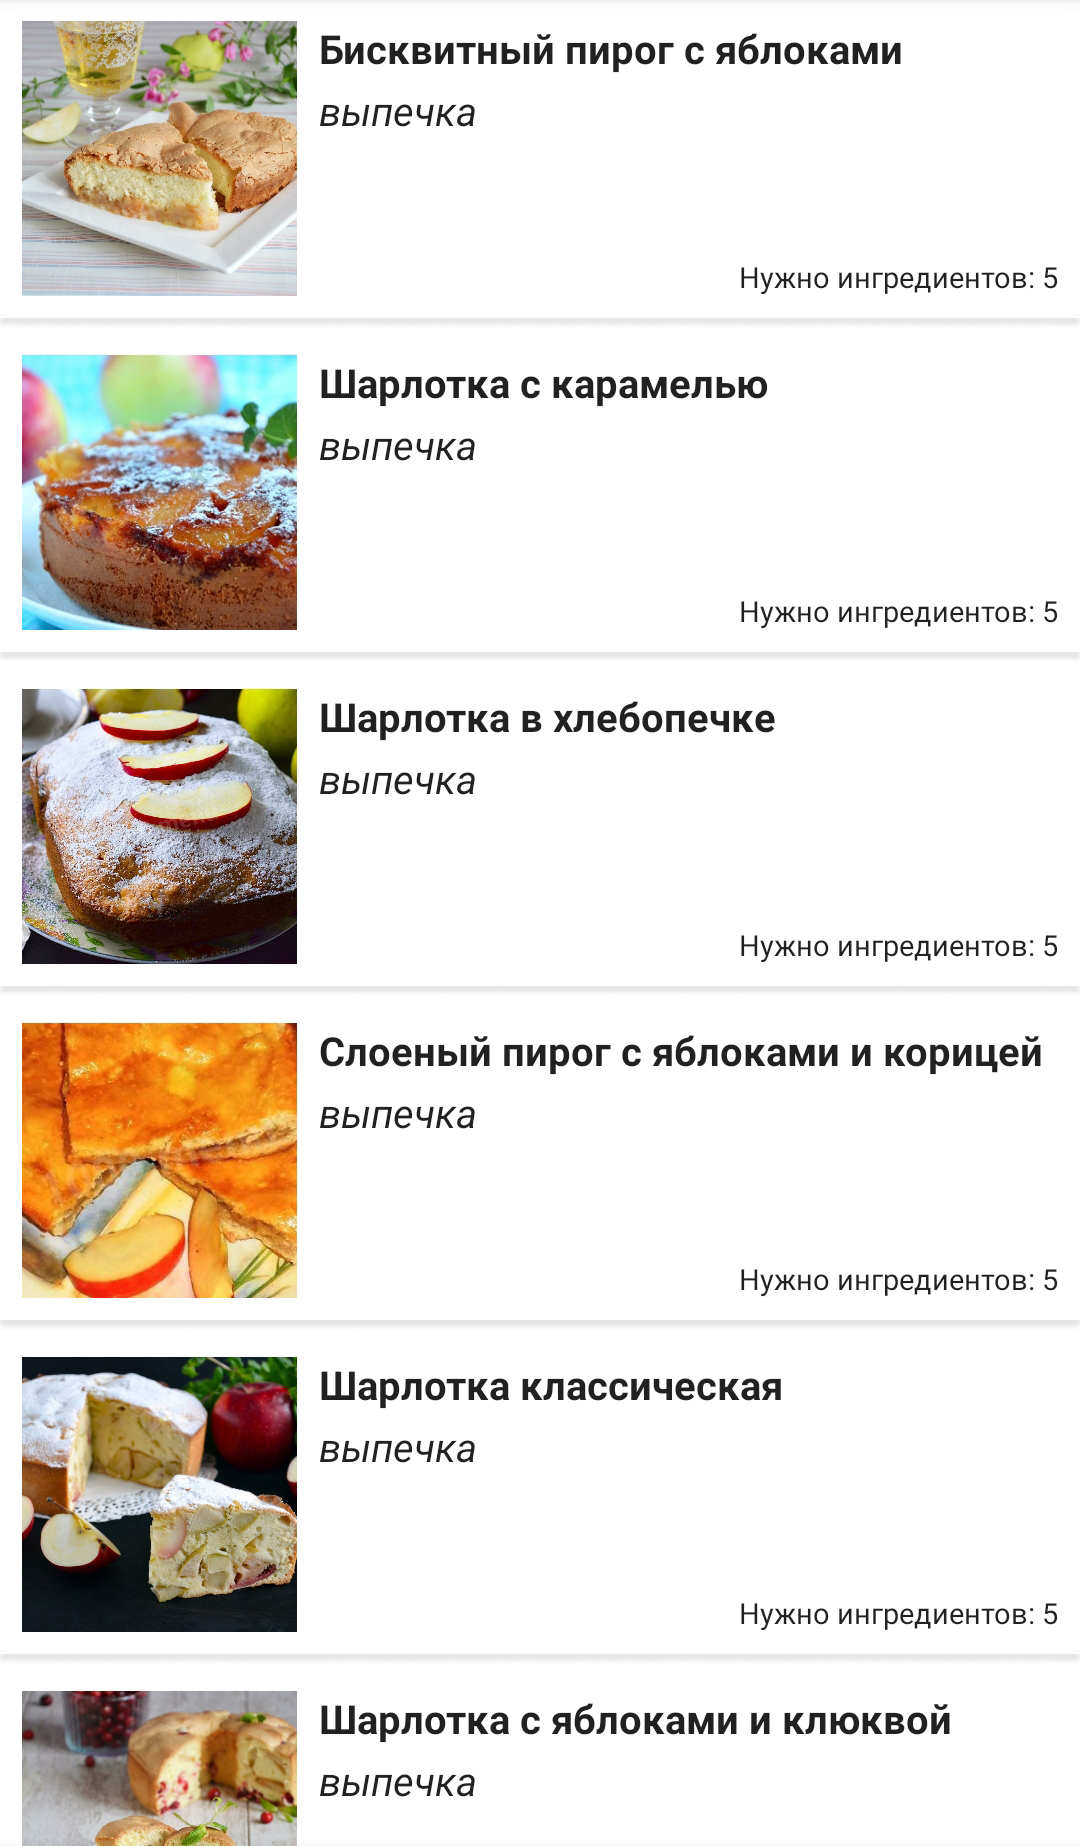
\includegraphics[scale=0.15]{resultpage.png}
\caption{Графический интерфейс фрагмента RecipeSearchResultsFragment}
\label{resultpage}
\end{figure}

\begin{itemize}  
\item \textbf{RecipeFragment} (Рис. \ref{recipepage}) Фрагмент отдельного рецепта, имеет вложенные фрагменты RecipeIngredientListFragment и\\ RecipeStepListFragment, отображающиеся в переключаемых вкладках и содержащие список ингредиентов и шаги приготовления соответственно. Так как приложение может инициировать перерисовку графического интерфейса фрагмента, данные о рецепте должны находиться в объекте, чьё состояние не зависит от таких изменений. Для этого существует библиотечный класс ViewModel, от которого в данном случае наследуется RecipeInfoViewModel, содержащий отображаемую информацию: название блюда, инструкцию и т. д.
\item \textbf{RecipeSearchResultsFragment} (Рис. \ref{resultpage}) Фрагмент со списком результатов поиска по запросу. Реализован при помощи компонента RecyclerView \cite{recycler}, использующего класс SearchResultsListAdapter для заполнения отдельного элемента списка соответствующими данными из базы.
\end{itemize}



\newpage
\section*{Результаты}

\begin{itemize}  
\item Спроектирована архитектура базы данных
\item Реализован инструмент для заполнения базы тестовыми данными
\item Реализован механизм доступа к данным
\item Реализованы элементы интерфейса для отображения результатов поиска
\end{itemize}

\setmonofont[Mapping=tex-text]{CMU Typewriter Text}
\bibliographystyle{ugost2008ls}
\bibliography{report.bib}
\end{document}
